\documentclass[11pt]{article}
\usepackage{fullpage}
\usepackage{graphicx}
\usepackage{natbib}
\usepackage{hyperref}
\usepackage{enumitem}

\begin{document}
\title{Analog Lab: Impedance, Filters, Amplifiers, and Noise}

\maketitle

The purpose of this lab is to learn some basic principles of electronic components
and circuits, as well as some laboratory methods.  The principles of impedance,
filtering, amplification, and noise are not only central to the operation of
radio telescopes, they are behind almost every modern technology you can think of:
radio, wifi, cell phones, speakers, \dots  you name it.  By the end of this lab,
you should be moderately comfortable using a multimeter, measuring RF signals,
building circuits, reading circuit diagrams, and poking around under the hood
of electronic gadgets.  You should also be able to describe mathematically how
impedances combine to make low-pass and high-pass filters, how random numbers
add together, and how noise is produced and passed along through a signal chain.
This lab runs for 3 weeks and covers a lot of ground.  Get ahead early.

\section{Week 1}
\label{sec:week1}
\subsection*{Prerequisites}

Reading: Horowitz \& Hill, Ch. 1

\begin{itemize}[noitemsep,nolistsep]
\item Ohm's Law
\item Th\'evenin Equivalent Resistance
\item Capacitance and Inductance
\item RC Filters
\item Diodes
\end{itemize}

\subsection*{Materials}

\begin{itemize}[noitemsep,nolistsep]
\item breadboard
\item misc R, C, L components
\item potentiometer (``pot'')
\item power supply
\item function generator w/ external FM reference
\item oscilloscope w/ probes
\item voltimeter
\item speaker w/ amplifier
\end{itemize}

\subsection*{Some Thoughts}

\subsubsection*{Breadboards}

Breadboards are convenient for constructing circuts for this lab.  Take some time to get to know yours
using a ohmmeter.  In particular, figure out what is connected, and what is not.

\subsubsection*{Grounding}

Ground means different things in different contexts (e.g. earth ground, signal ground,
chassis ground).  For our purposes in
this lab, ground simply provides a return path for current.  We define it to be
0V (i.e. it is the reference from which we measure voltage differences).  The
ground of your circuit should be tied to the ground of your power supply.  It
is good practice to consistently use a color (black, blue, and green are good
choices) to indicate ground lines in your circuits.

\subsubsection*{Capacitor Orientation}

Some capacitors, particularly electrolytics, care about which direction voltage
is applied across them.  Often, one of the leads is longer, and may have a `+'
near it on the body of the capacitor.  Always connect this lead to the higher voltage.
Failure to do so can, for higher voltages, cause them to explode.

\subsubsection*{Oscilloscopes}

'Scopes can be intimidating.  The solution is to press buttons until they submit.  Seriously, don't be afraid
to push buttons.  In order to show a static display of a repeating signal, scopes need to trigger on
some edge of an input signal.  This is always configurable, and you'll need to figure out how.  You can
adjust the time (X axis) and voltage (Y axis) ranges, and should do so regularly.  Many scopes have an ``auto''
button, which is a totally useful cop-out.  Probes that connect to the scope often amplify
(10:1), and scopes have a setting to undo this for the display.  Finally, there is a difference between
attaching a probe and attaching a cable.  This difference has to do with termination.  We haven't covered yet
what termination is (it's next week), but suffice it to say that in order for your voltage scale to mean
something, you should select 50$\Omega$ if you have connected a cable (BNC, SMA, etc.), and 1M$\Omega$ if
you are using a probe.

\subsubsection*{FM Radio}

\begin{figure}[h]
\centering
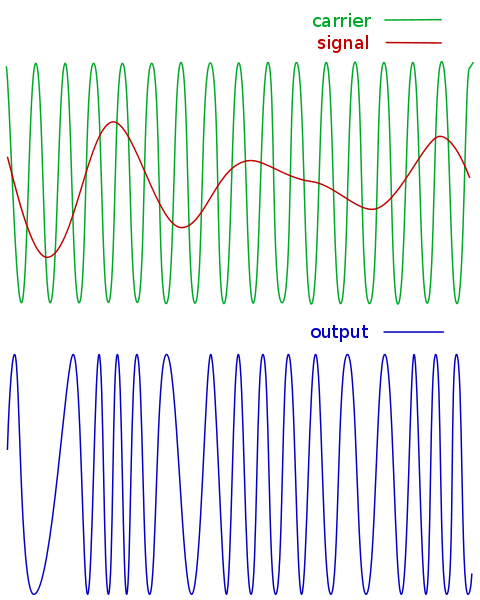
\includegraphics[width=3in]{plots/frequency_modulation.png}
\caption{Frequency modulation}\label{fig:frequency_modulation}
\end{figure}

Frequency modulation (FM, see Figure \ref{fig:frequency_modulation}) is a clever scheme for 
encoding a signal.  Amplitude modulation (AM) radio
directly mixes a carrier tone with a signal, so that the amplitude of the signal creates an envelope inside
of which the carrier tone oscillates.  FM instead translates the amplitude of the signal into a change
in the frequency of the carrier tone (see above).  FM radio stations typically transmit between 88 and 108 MHz
in the US.  However, for the purpose of this lab, owing to lack of radio reception in the lab, and the
difficulty in using discrete components at higher frequencies, we will create our own radio station at
1.045 MHz, instead of 104.5 MHz.  Typically, FM radio stations are spaced every 200 kHz, and have a frequency
deviation of $\pm$75 kHz at maximum scale input.

\subsection{Resistive Voltage Divider}

\subsubsection{Useful Equations}
\begin{equation}
V=IR
\end{equation}
\begin{equation}
P=IV
\end{equation}

\subsubsection{Activities}
\begin{itemize}[noitemsep,nolistsep]
\begin{figure}[h]
\centering
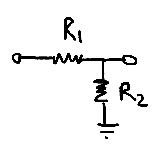
\includegraphics[width=2in]{plots/volt_divider.png}
\caption{A voltage divider}\label{fig:volt_divider}
\end{figure}
\item build voltage divider (Figure \ref{fig:volt_divider}) out of two 1k resistors, 
connect input to +5V DC voltage source
\item measure voltage at output
\item measure current (think carefully about where before burning out the multimeter fuse!)
\item apply 1 MHz sine wave, view input and output on oscilloscope
\item append a second voltage divider to the output of the first (choose resistor values carefully)
\item for a voltage divider, is it better to have high impedances or low?  what considerations might
drive you in either direction?
\item from the perspective of the second voltage divider, what is the Th\`evenin equivalent resistance
of the first divider, as seen from its output?
\begin{figure}[ht!]
\centering
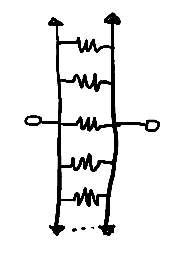
\includegraphics[width=1.5in]{plots/resistor_series.png}
\caption{An infinite series of resistors}\label{fig:resistor_series}
\end{figure}
\item if each resistor in Figure \ref{fig:resistor_series} is the same value, what is the equivalent resistance
between the two terminals?  (BTW, I still haven't solved http://xkcd.com/356, but don't get nerd sniped
while doing this lab!)
\end{itemize}

\subsection{Capacitive Voltage Divider}

\subsubsection{Useful Equations}
\begin{equation}
I=C\frac{dV}{dt}
\end{equation}

\begin{equation}
Z_C = \frac1{j\omega C}
\end{equation}

\subsubsection{Activities}

\begin{itemize}[noitemsep,nolistsep]
\item build a voltage divider out of two 1$\mu$F capacitors, connect input to 1 MHz sine wave
\item compare input and output on oscilloscope.  is it what you expected? what is the DC level at the output?
resistor?
\item add a 1k resistor to ground at the output, and then for your modified circuit, graph the 
expected $V_{out}/V_{in}$ versus frequency
\end{itemize}

\subsection{RC filter}

\subsubsection{Activities}
\begin{itemize}[noitemsep,nolistsep]
\item design a high-pass filter with cutoff (-3dB) at 100 kHz
\item design a low-pass filter with the same cutoff
\item plot the expected responses of each.  spot-check with oscilliscope measurements.
\item what could you do to get steeper transitions in RC filters such as these?
\end{itemize}

\subsection{LC filter}

\subsubsection{Useful Equations}
\begin{equation}
Z_L = j\omega L
\end{equation}

\begin{equation}
Q = \omega_0 RC = \frac{f_0}{\Delta f_{3dB}}
\end{equation}

\subsubsection{Activities}
\begin{itemize}[noitemsep,nolistsep]
\begin{figure}[h]
\centering
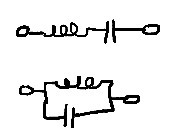
\includegraphics[width=2in]{plots/lc_series_parallel.png}
\caption{An inductor in series and in parallel with a capacitor}\label{fig:lc_series_parallel}
\end{figure}
\item plot the theoretical impedance versus frequency of a 1 $\mu$H inductor in parallel 
with and in series with a 1 $\mu$F capacitor (Figure \ref{fig:lc_series_parallel}).
\begin{figure}[h]
\centering
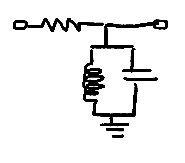
\includegraphics[width=2in]{plots/rlc_filter.png}
\caption{A bandpass RLC filter}\label{fig:rlc_filter}
\end{figure}
\item design and build an LC band-pass filter (Figure \ref{fig:rlc_filter}) tuned to 1 MHz
\item choose an R to select a quality factor appropriate for $\Delta f_{3dB}=200 kHz$.
%\item for a moment, swap out your C for something quite small (say, 100 pF) and measure empirically
%the frequency of peak response.  assuming your inductor value is correct, what is your inferred capacitance?
%if this doesn't agree with your C, can you explain why?
\end{itemize}

\subsection{Diodes}

\begin{itemize}[noitemsep,nolistsep]
\item measure the voltage drop over a conducting diode (important: limit current flow with a resistor!)
\item use different resistor values (or a pot) and measure the voltage drop as a function of current
\item use a large ($\pm$ 1V) oscillating signal into the diode and view the original and rectified 
signal on an oscilloscope
\item apply a low-pass filter with time constant of order the input frequency, and view the 
output on an oscilloscope.  generate a plot of what is going on here.
%\item suppose you have an oscillating signal whose amplitude is less than the voltage drop across your conducting
%diode.  can you come up with a circuit that re-centers your oscillating signal on the threshold 
%of diode conduction?
\end{itemize}

\subsection{FM demodulation}
\begin{figure}[h]
\centering
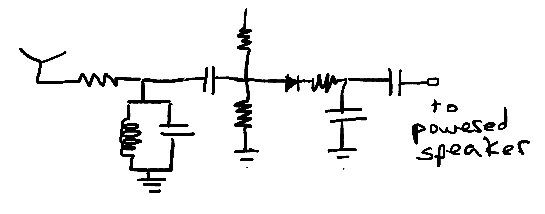
\includegraphics[width=4in]{plots/fm_demodulation.png}
\caption{An FM demodulation circuit}\label{fig:fm_demodulation}
\end{figure}

\begin{itemize}[noitemsep,nolistsep]
\item use your LC circuit to convert a frequency-modulated signal into an amplitude modulated signal
\item use your diode circuit as an "envelope detector" that filters out the carrier frequency and extracts the
amplitude modulation.  Use a 100 kHz low-pass filter in the envelope detection. (Humans can only hear up to 40 kHz
or so).  You should have something like Figure \ref{fig:fm_demodulation}.
\item connect in our faked FM station at 1.045 MHz
\item connect the output through a coupling capacitor (to remove the DC bias) to amplifying audio speakers
\item enjoy listening to the music
%\item fun part: which components of your circuit are strictly necessary?  try removing some of them and see
%if it still works?  Draw your circuit as it worked before and after ``contracting'' it.
%\item if our station is at 1.045 MHz, why is your LC tuned to 1.0 MHz?  %what was relevance of the quality factor?
\end{itemize}

\subsection{For Your Report}
\begin{itemize}[noitemsep,nolistsep]
\item Present a circuit diagram of an FM radio receiver, highlighting blocks 
of components that act as a unit to perform some action (filtering, biasing, etc.)
\item Describe in the text the overall design of the FM receiver, with subsections for each
functional block, listing salient features of each (e.g. the -3dB point of a filter,
the voltage biased to, etc.).  Present it as if you invented it, and were writing the seminal
paper that will enable others to use this design.
\item Using your new understanding of impedances, plot the expected output of the LC filter in
your FM receiver as a function of frequency, $f=\omega/2\pi$.  Mark the location, in frequency, 
of the transmission band used in the lab, and explain the rational behind its placement on the LC
response curve (e.g. if our station is at 1.045 MHz, why is your LC tuned to 1.0 MHz?)
\item Finally, also plot, as a function of frequency, the bandpass of the final filter that
defines the band of the output audio signal.  Describe (and maybe plot) the rationale for
selecting the filter that you did.
\end{itemize}

\section{Week 2}
\label{sec:week2}
\subsection*{Prerequisites}

Reading: Horowitz \& Hill, Ch. 2

\begin{itemize}[noitemsep,nolistsep]
\item Transmission Lines
\item Transistors
\item Amplifier Circuits
\end{itemize}

\subsection*{Materials}

\begin{itemize}[noitemsep,nolistsep]
\item rope and string of various thicknesses (pretty long)
\item breadboard
\item misc R, C, transistor components
\item power supply
\item function generator w/ external FM reference
\item oscilloscope w/ probes
\item voltimeter
\item speaker w/o amplifier
\item long cable (as long as possible, longer than 100m would be great)
\end{itemize}

\subsection*{Some Thoughts}

\subsubsection*{Transistors}

\begin{figure}\centering
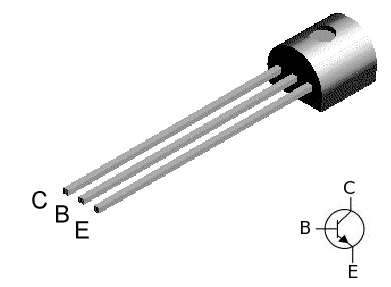
\includegraphics[width=2in]{plots/npn_transistor_pins.png}
\caption{Pinout for a generic NPN transistor (e.g. 2N3904)}
\label{fig:npn_transistor_pins}
\end{figure}

We'll be using an NPN bipolar junction transistor in this lab (see Figure \ref{fig:npn_transistor_pins}).  With
the flat face to you, pins typically read, from left to right, emitter, base, collector.  Now you know.

\subsubsection*{Speakers}

Last week, we just stuck our signal into an amplifying speaker and didn't think much about it.  This weak, since we are building our own amplifier, you might be wondering what's left that makes a ``speaker.''  Speakers aren't
that complicated.  At their simplest, they are solenoids that push/pull on a small magnet
attached to a diaphram.  Depending on which direction current is made to flow through the solenoid by an
alternating voltage signal, a magnetic field is set up that attracts or repels the magnet on the diaphram.  The
diaphram translates the resulting motion into pressure waves that propagate through the air.

\subsubsection*{Termination}

At the end of this lab, we'll be playing with some 50$\Omega$ (and maybe some 75$\Omega$) cable, examining how
waves are reflected and transmitted.  Of course, now you also have a better idea of why the oscilloscope
has selectable termination, and why it might be different depending on whether you connect as scope probe
or a BNC cable to the input.  Now that you know why and how, you have no excuse not to exercise good termination
practices!

\subsection{Impedance Mismatches on Rope}

\begin{itemize}[noitemsep,nolistsep]
\begin{figure}[h]
\centering
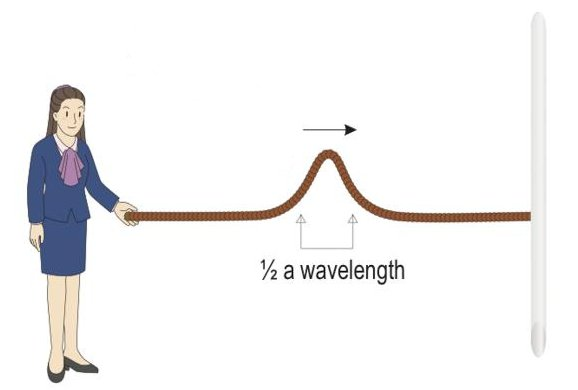
\includegraphics[width=2in]{plots/rope_pulse.jpg}
\caption{Sending a pulse down a rope}
\end{figure}
\item Get several lengths of ropes of different thicknesses.  Tie them together and tie the end of the thinner
rope to a doorknob or some other stable structure.  Hold the untied end, pull the rope relatively taut, and
then, with a quick up-down movement of the hand, send a pulse down the rope.  Observe what happens at
the interface between the ropes, and at the doorknob.
\item Switch the rope around so that the thicker end is now tied to the doorknob.  Repeat the above.  Any
difference?  
\item What would happen, do you think, if the far end of the rope, instead of being tied to a fixed point,
was tied to a ring that could move up and down on a pole?
\item Any idea how to stop the wave from reflecting off the far end of the rope?
\item If you have two thick ropes joined by a very short thin piece (small with respect to the
wavelength of the signal), what happens at that interface?
\item What about vice versa (thin ropes joined by a short thick piece)?
\end{itemize}

\subsection{Impedance Mismatches in a Transmission Line}

\begin{itemize}[noitemsep,nolistsep]
\item Get a function generator that can output square waves.
Get a long stretch of cable and connect the function generator output to one
end of the cable.  Leave a point that you can probe with an oscilloscope.
\item Use an oscilloscope to try to detect the reflected wave.  Draw the superposition of 
transmitting and reflecting waveforms that produces your output.
\item How long is your cable?  How fast did your
pulse travel?  (BTW, it can be helpful to know that, round-about, light travels 1 ft in 1 ns, and that
waves on a cable can be up to a factor of 2 slower than that.)
\item Use a 10$\Omega$ resistor to terminate the far end of the cable.  Observe the change.
\item Now properly terminate the far end, and recover your waveform!  What was the impedance of the cable?
\end{itemize}

\subsection{Building an Follower}

\begin{figure}[h!]\centering
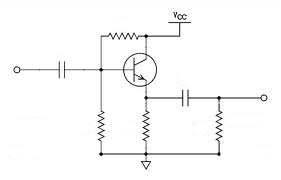
\includegraphics[width=3in]{plots/biased_emitter_follower.png}
\caption{An emitter follower that uses a biasing circuit.}
\label{fig:emitter_follower}
\end{figure}

\begin{itemize}[noitemsep,nolistsep]
\item Build the emitter-follower circuit shown in Figure \ref{fig:emitter_follower}, choosing approprite
values for resistors and capacitors.  Use a 2N3904 transistor, or a similar substitute NPN BJT.  You will
power the circuit with $V_{cc}=+5V$, and will want to amplify signals in the range 100Hz to 50kHz.  Mind
your R's and C's!
\item Measure the bias voltage $V_{BE}$.
\item What is the purpose of the emitter resistor (that is, the resistor most immediately connected to the
emitter)?
\item Input a 10 kHz sine wave with 1V amplitude.  What is the relationship between the input and output voltages?
\item Predict first, and then measure, the maximum sine amplitude for which this circuit correctly operates.
\item Measure the bias voltage at the base.  How small can you make the emitter resistor before it changes?  You
might need to make the resistors in your bias circuit large so that you don't burn up the emitter resistor.
\end{itemize}

\subsection{Building an Amplifier for our FM radio}

\begin{figure}[h!]\centering
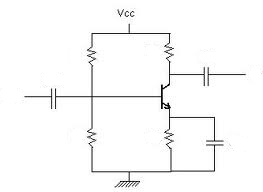
\includegraphics[width=3in]{plots/bjt_amplifier_lab2.png}
\caption{An amplifier based on an NPN BJT.}
\label{fig:amplifier}
\end{figure}

\begin{itemize}[noitemsep,nolistsep]
\item Build the amplifier circuit shown in Figure \ref{fig:amplifier}, choosing appropriate values for
resistors and capacitors, using the same constraints as for the follower circuit above, and choosing a
DC gain of 2.  For the time being, omit the emitter capacitor.
\item What is the voltage at the collector?
\item Input a 10 kHz sine wave with 100mV amplitude.  What is the relationship between the 
input and output voltages?  If you did not achieve a gain of 2, why not?
\item Predict first, and then measure, the maximum sine amplitude for which this circuit correctly operates.
\item Now add in the emitter capacitor to select for a gain of 10 at 10kHz.  Again, mind your R's and C's!
\item Input a 10 kHz sine wave with 100mV amplitude.  What is the relationship between the 
input and output voltages?  If you did not achieve a gain of 10, why not?
\item Predict first, and then measure, the gain at 20 kHz.
\item Can you think of a way to make this circuit have the same gain across our whole band of interest?
\item Finally, attach a passive speaker to the output, your passive FM demodulator to the input, and bask in
the sound of your success.  You'll need to pay attention to the impedance of the speaker, and plan accordingly.
\end{itemize}

\subsection{For Your Report}
\begin{itemize}[noitemsep,nolistsep]
\item Add a section describing your speaker amplifier, including a circuit diagram, and describing
how it functions (and what the various functional parts are).  I'll be looking for a description
of how the base and collector voltages are set, and why they needed to be set where they are.
\item Specify the input and output impedance of your circuit at audio ($\sim$10 kHz) frequencies.
\item Suppose your speaker amplifier connects to a speaker at the end of a long run of wire.
Given the amplifier circuit that you built, what impedance cable to you recommend, and how would you
terminate it (incorporating an 8-Ohm speaker) to avoid reflections?  For now, don't worry, unless you want
to, about maximizing the current through the speaker (to make it LOUD).
\item Define the operating band of your amplifier.  Over what frequency ranges does it operate,
and what specifically determines the bounds on this range?
\end{itemize}

\section{Week 3}
\label{sec:week3}

\subsection*{Prerequisites}

\begin{itemize}[noitemsep,nolistsep]
\item Central Limit Theorem
\item Johnson-Nyquist Noise
\item Receiver Temperature
\item Radiometer Equation
\end{itemize}

\subsection*{Materials}

\begin{itemize}[noitemsep,nolistsep]
\item 2W 50$\Omega$ resistor
\item power supply
\item oscilloscope w/ probes
\item minicircuits amplifiers
\item voltimeter
\item infrared (remote) thermometer
\end{itemize}

\subsection*{Some Thoughts}

\subsubsection*{Minicircuits Amplifiers}

Now that you've built your own amplifier, you have a feel for what goes on inside an amplifier.  We're
now going to use pre-packaged amplifiers that are commercially available (Minicircuits is a typical vendor).
These will be SMA in, SMA out, with two leads for $V_{cc}$ (+15V, for the parts we're using) and ground.
These amplifiers specify their gain in dB, and you do have to be a bit careful about signal levels.
As a general rule, the output of amplifiers should be connected (to a 50$\Omega$ load) before they are
powered on, so that they don't have to dissipate their output power internally.

\subsubsection*{Infrared Thermometer}

If you assume that objects radiate heat as a blackbodies (which we'll discuss in later labs), you
can measure their temperature remotely just by their infrared radiation.  The infrared thermometer
we will use in this lab is an infrared telescope (with a well-defined beam size) that is
calibrated to output a voltage in mV that is the temperature in Fahrenheit.  Use it wisely.

\subsubsection*{Interference}

In this lab, we're going to attempt to make a relatively sensitive measurement of the Johnson
noise on a 50$\Omega$ resistor.  It turns out that lots of things can produce signals at this 
level that can interfere with your measurement.  For one, if you make a loop that electrons can
flow around (which, after all, is what a circuit is), then a changing magnetic flux through that
loop produces an EMF that drives a current that sets up a voltage across the resistor.  This may
be the very first radio antenna we build in this class.  Unfortunately, that's not what we were
going for, so we need ways to avoid this.  Since the area inside the loop matters, you can try to
make your circuits physically narrow.  You might also try making a Faraday cage.

\subsubsection*{Writing Code for Lab}

This is the first lab where a significant portion of the lab is writing code. 
So the first thing you should do set up a github
account and start a repository that will contain all the code you turn in for this class (and
while you're at it, why not your \LaTeX reports too?).
Next, clone your repo onto your computer.  (If you haven't yet, you should get Git, Python, Numpy,
and Pylab installed).  Inside your repository, add a directory ``lab\_analog", and create
%two files: central\_limit.py and radiometer\_test.py.  Commit, and push your changes back up to
the file: central\_limit.py.  Commit, and push your changes back up to
your github account.  Inside your lab report, make sure you link to your repository in
your ``Methods" section, along with the hash tag that indicates which commit was the one used
to produce your results.  

\subsection{Calculating the Noise Figure of a Reciever}

\subsubsection*{Determine Amount of Gain Needed}
\begin{itemize}[noitemsep,nolistsep]
\item Calculate how much amplification is needed to bring the Johnson noise on a $50\Omega$ resistor
up to at least the $\sim$1mV RMS level that you can measure on a scope.  You'll have to pick an appropriate
bandwidth, and you might want to check that you can get a filter that supplies that bandwidth. 
\item Looking at the data sheets for the minicircuits amplifiers, choose a number of gain stages.
\item Connect the gain stages (and the filter at the end), and power them at +15V.  IMPORTANT: Most amplifiers
want to have the output connected first, so that the output power has some place to go.
\end{itemize}

\subsubsection*{Estimate and Measure the Resistor Temperature}
\begin{equation}
P=A\epsilon \sigma T^4
\end{equation}
\begin{itemize}[noitemsep,nolistsep]
\item Set a power supply to the appropriate voltage to dissipate $\sim$2W in a 50$\Omega$ resistor (make
sure it is a beefy resistor rated to 2W, and do not exceed that threshold, or meltdown will ensue).
\item Using the Stefan-Boltzmann Law, calculate what temperature you think the resistor will hit.
\item Use an infrared thermometer to measure the temperature.  Were you close?
\end{itemize}

\subsubsection*{Measure the Noise Figure}
\begin{itemize}[noitemsep,nolistsep]
\item Determine the power out of the receiver for the input resistor at room temperature.  Ideally, you'd do this
with a power meter or a spectrum analyzer, but today, we'll do the poor man's method of eyeballing one
standard deviation from the mean on an oscilloscope.  This isn't easy, and I apologize for that.  To keep your
sanity, you should estimate errorbars on this measurement, so you can see the effect of error on
your bottom line.
\item As in the previous step, set the resistor dissipating 2W, and measure the power out of the receiver.
IMPORTANT: Use a blocking cap to prevent a large DC voltage from entering the amplifier chain.  Otherwise, you
could damage your amplifiers.  When in doubt, ask.
\item Since you already know the temperature the resistor hits when dissipating 2W, you should be able to
solve for the gain and the receiver temperature (and if you want, you can calculate your Y factor).  This
would be a good time to use your error bars to determine your confidence interval on your measurement
of the gain and receiver temperature.  Make a plot and draw some lines!
\item Convert your receiver temperature to a noise figure.
%\item How much is your error on the receiver temperature reduced if you have a prior on the gain (which
%you should look up from the data sheet)?
%\item How does your measured receiver temperature compare to the noise temperature you'd expect given
%your chain of amplifiers? 
\end{itemize}

\subsection{Demonstrate the Central Limit Theorem}
\begin{itemize}[noitemsep,nolistsep]
\item Write a program (in the central\_limit.py file that you created earlier)
that shows that, in the large-N limit, adding samples drawn from non-Gaussian random
distributions converges to a Gaussian distribution.
\item Also show that the standard deviation of the mean of $N$ Gaussian-random samples decreases as $\sqrt{N}$.
If you are trying to characterize samples of an unknown character to show that they are noise-like, this
is called an Allen variance test.
\end{itemize}

%\subsection{Numerical Demonstration of the Radiometer Equation}
%\begin{itemize}[noitemsep,nolistsep]
%\item Write a program (in the radiometer\_test.py file) that simulates 
%random noise corresponding to a noise temperature, and shows that the radiometer equation works.  In particular,
%prove (numerically) that it is, in fact, $\sqrt{Bt}$ and not $\sqrt{2BT}$ in the denominator of the
%radiometer equation.
%\end{itemize}

\subsection{For Your Report}
\begin{itemize}[noitemsep,nolistsep]
\item Pretend that the amplifier whose noise figure you were determining was the one you built
in \S\ref{sec:week2}.  Describe the methodology for determining the noise figure, including
the relevant equations used.
\item Report the final noise figure you measured.  Give error bars.  What are your sources of error?
\item One last charade.  Let's say that you also wanted to test how the noise output by your
amplifier integrates down, to be sure that there are no systematics present.  Pretend you placed a
known-good noise source in front of your amplifier and digitized the output of your amplifier, and you
get the numbers output by your central\_limit.py program.  Perform an Allen variance test to show
that the noise from your amplifier behaves as you'd expect.  Produce a plot of variance (or standard deviation,
either one) versus number of samples averaged, along with the slope of the line you're shooting for.
\end{itemize}

\end{document}
